
\documentclass[master]{thesis-uestc}

\title{快速近似图模式挖掘系统关键技术研究}{A Research of technologies of 
fast approximate graph pattern mining system}

\author{王亦君}{Yijun Wang}
\advisor{薛瑞尼\chinesespace 副教授}{Dr. Ruini Xue}
\school{计算机科学与工程学院}{School of Computer Science And Engineering}
\major{计算机科学与技术}{Computer Science and Technology}
\studentnumber{201421040223}

\begin{document}

\makecover

\begin{chineseabstract}
为了适应日益增长的宽带信号和非线性系统的工程应用,用于分析瞬态电磁散射问题的时域积分方程方法研究日趋活跃。本文以时域积分方程时间步进算法及其快速算法为研究课题,重点研究了时间步进算法的数值实现技术、后时稳定性问题以及两层平面波算法加速计算等,主要研究内容分为四部分。

……

\chinesekeyword{时域电磁散射,时域积分方程,时间步进算法,后时不稳定性,时域平面波算法}
\end{chineseabstract}

\begin{englishabstract}
With the widespread engineering applications ranging from broadband signals and non-linear systems, time-domain integral equations (TDIE) methods for analyzing transient electromagnetic scattering problems are becoming widely used nowadays. TDIE-based marching-on-in-time (MOT) scheme and its fast algorithm are researched in this dissertation, including the numerical techniques of MOT scheme, late-time stability of MOT scheme, and two-level PWTD-enhanced MOT scheme. The contents are divided into four parts shown as follows.

\englishkeyword{Time-domain Electromagnetic Scattering, Time-domain Integral Equation, Marching-on In-time (MOT) Scheme, Late-time Instability, Plane Wave Time-domain (PWTD) Algorithm}
\end{englishabstract}

\thesistableofcontents

\chapter{绪\hspace{6pt}论}

\section{研究工作的背景与意义}

    随着互联网的高速发展,数据量呈指数级爆发式增长。有效处理不同类型的数据至关重要。
海量数据中有很大一部分的数据由不同个体间的交互产生,这种互相关联的数据天然适合
图(Graph)数据结构~\cite{NetworkScience}。图是由顶点(Vertex)和边(Edge)组成。
将实体信息存储为顶点,将它们之间的关系转换为边,则可以通过研究分析图的拓扑和度量来
直接探索数据之间的相关性。如何发现图数据间的联系是一个普遍的问题,被称为图挖掘(Graph Mining)。

    模式挖掘(Pattern Mining)是图挖掘中一项主要的任务,其主要目的是从图数据中找到
特定的子图结构,这样的子图结构称为模式(Pattern)。模式挖掘中的关键算法是“模式计数”。
研究证明,确定一个子图是否存在于另一个更大的图数据集中(即子图同构)是一个NP完全问题~\cite{Complexity}。
而更进一步精确计算出该子图的出现次数(即模式计数)则更加困难。最直观的方法是精确的执行算法,
但这带来了很大的计算资源消耗,即使在相对较小的图数据集中,也会出现数百万甚至数十亿的同构子图。
例如,在一个由20个节点组成的集群中,分布式GPM框架Arabesque~\cite{Arabesque}需要10个多小时才能在
一个有10亿条边的图形中计算三角形,这在许多情况下都是不可接受的。

    随着数据量的爆炸增长,精确的模式计数越来越变得困难。当前很多数据分析应用要求接近实时的响应速度
,精确方法面临着响应慢的问题。而通过观察分析,许多模式挖掘应用并不需要查询出与模式图匹配的每一个真实
子图,例如:频繁子图挖掘是找出特定模式的出现频率并筛选出频率较高的子图,这种情况只需要筛选出频率超过
特定阈值的子图即可,并不需要完全准确的结果;得出数量级接近的结果即可。因此,近年来许多图挖掘研究运用
近似理论,寻求在保证结果一定程度精确性的前提下大大提高计算效率~\cite{BlinkDB,GRASS}。
图近似挖掘的基本思想是通过采样手段缩减数据集的规模,在样本上执行精确算法,通过采样概率来估算原本数据
集中真实结果~\cite{Congressional}。ASAP~\cite{ASAP}提出了一种基于边缘采样的近似方法,与Arabesque
相比性能提高了两个数量级,并且保证误差低于5\%。

    真实的图数据集往往呈现幂律分布特征~\cite{LargeScale}。图数据的幂律分布特征是指度数和度数对应得
顶点数呈幂函数关系,即度数$d$和顶点数$v_{\#}(d)$有:$v_{\#}(d)=c \cdot d^{-k}$,该式展示了少量的
高度数的顶点连接大量边的现象。对于模式挖掘来说,不同度数的顶点对于模式的贡献有很大不同,针对数量稀少
连接边却很多的高度数节点和数量庞大连接边较少的低度数节点采用不同的采样频率,能够达到缩短查询时间、
减少查询误差的目的。

    近似图模式挖掘中应用幂律特性分析,需要在具体模式挖掘应用执行前进行图数据预处理:获取幂律分布函数
基本参数,按度数信息处理节点集和边集,方便后续基于幂律特性的近似挖掘算法运行。这一部分预处理带来一定
的时间开销。但是ASAP等目前的图近似挖掘算法在采样之前不对数据本身做处理,采样时使用原始的边流进行采样,
这样带来了很大的采样开销。通过预处理技术可以提前获取数据集中边分布信息,加速采样过程,有效地降低采样开
销。与之相较,进行幂律分析的预处理技术带来的开销是非常值得的,并不会使预处理时间变得难以接受。



\section{国内外研究历史与现状}
\subsection{图模式挖掘研究现状}
    图数据是一种灵活的数据结构,能够用于建模真实世界事物之间的联系。图常常被用于分析万维网的结构
~\cite{WebgraphFramework},生物信息学数据~\cite{DeNovo},化学中的原子和共价关系~\cite{Chemistry}
等等领域的数据。从图数据中提取信息成为了一个重要的研究领域~\cite{NetworkScience}。许多研究者和Facebook
、谷歌等互联网企业,推出了自己的图数据系统来处理数据中的关联,例如具有数十亿个顶点和数千亿条边的Facebook
用户图。

    图挖掘使用数据挖掘技术在给定的图数据集中查找模式或关系。通过挖掘图,可以识别频繁的子结构和关系,
这有助于对图集进行聚类,找到图集之间的关系,或者识别或描述图。图挖掘过程中,寻找图中频繁出现的
模式十分重要。

    在图模式挖掘的典型应用中统计模式的出现频率非常常见,模式计数算法正是其中的重点。
随着图模式挖掘多年来的发展,许多计数算法和方法被开发出来,其中主要分为两大类,精确计数和近似计数。

    精确计数确定查询模式的准确频率。给定一个k大小(k个顶点)的模式,经典算法首先枚举具有k个顶点的所有连通子图,然后使用图同构算法对子图
进行分类以找到特定的模式。MFinder~\cite{Motifs}提出一种边扫描法,将以下步骤应用于图的每条边:维护一个集合$S$中,如果扫描到的边不在$S$中但与$S$中
至少一条边相连接,则将边加入$S$。当$|S|=k$时,通过维护找到的子图的哈希表,判断是否第一次找到了由$S$诱导的子图。在经典方法的基础上,
Grochow和Kellis~\cite{MotifUseSymmetryBreaking}提出了一种高效的单模式搜索方法,运用对称破缺的方法防止自同构的模式被重复计算。
这种防止重复计算的思想更进一步发展,出现了利用模式的常见拓扑特征或提取模式特征的封装方法。例如,Ribeiro和Silva~\cite{GTries}设计了图的前缀树。
树的每个节点表示一个不同的图,其中父节点及其子节点共享一个公共子结构。然后,它从前缀树的根搜索所有同构模式。近年来,出现了分解方法,
主要思路是识别每个计数模式的子结构,将它们划分为更小的模式分别进行计数。Pinar等~\cite{ESCAPE}于2017年提出将顶点数为5的模式分解为子结构然后进行计数,
并且描述了如何通过公式计算原本大小为5的模式频率。

    由于精确计数的计算复杂性,研究者针对大型图提出了各种近似计数方法~\cite{SampleInBigGraph}。其主要思想是通过采样生成一个简化子图,在子图精确计算模式,
然后缩放子图结果以估计最终结果。Lim等人~\cite{MemoryEfficient}以固定概率对边进行采样,并在采样边后检查模式。它不需要图的任何其他先验知识,
并使用Bloom过滤器检查重复的边。FURL~\cite{FURL}和PartitionCT~\cite{PartitionCT}将为边分配$rank$,并将其散列到大量的存储桶中。
每个桶只保留$Rank$最小的边缘。存储新边后,他们会搜索它是否可以与其他桶中的边形成模式。处理完所有边后,子图结果用
HyperLogLog~\cite{HyperLogLog}缩放,以估计整个图中的实际模式数。SWTC~\cite{SlidingWindow}提出了一种基于滑动窗口的算法,
用于对具有重复边流的图中三角形进行近似计数。SWTC的核心是一种固定长度切片策略,它在有限内存使用情况下解决了无偏采样和基数估计问题。
ASAP~\cite{ASAP}同时启动了大量的估计量,以便对图形进行统一采样。每个估计器执行邻域采样算法,并用贝叶斯概率估计模式数。最后,
ASAP汇总所有估计器的结果。创建的估值器越多,准确度就越好。ASAP提供ELP(错误延迟配置文件),允许用户平衡计算成本和结果准确性。

    所有近似计数方法都会进行某种采样,并且所有方法都平等地考虑顶点和边。也就是说,图是均匀采样的,这实际上没有考虑大多数图的幂律特性。

\subsection{幂律图研究现状}
    幂律分布是一种普遍存在的现象~\cite{PowerlawBrief},早在20世纪50年代,已经在生物学~\cite{Stochastic}、经济学~\cite{Zipf}等领域被发现,比如幂律分布适用收入分配模型的讨论。
而计算机领域对于幂律图的研究源于对互联网网络拓扑的观察~\cite{Statistical}。Faloutsos、Faloutoss和Faloutos~\cite{faloutsos1999powerlaw}将互联网
看作一个无向图,用图中的每个顶点表示路由节点,他们从图的结构中发现了幂律分布。并且他们发现不仅仅是大规模互联网,在不同规模的节点之间的关系,
从局域网上的主机联系到整个互联网所涵盖的范围都体现了幂律规律,这说明了幂律规律的适用性非常广泛。之后,用图结构来组织社交网络~\cite{Characterization}、
运输网络~\cite{Transportation}、商业竞争合作关系~\cite{Company}等等数据的时候,这些图数据也普遍显示出幂律分布特征。

    对于图数据幂律特性,有很大一部分相关研究运用数学理论分析进行理论分析~\cite{clauset2007powerlaw}。许多图算法利用分布特征进行优化:
Abou-Rjeili等人~\cite{MultilevelPartitioning}针对幂律图改进了图的多级划分算法;Fan Chung等提出了一种计算幂律图的邻接矩阵的最大特征值的方法~\cite{Eigenvalues}。
Perseus~\cite{Perseus}是一种大规模图挖掘和可视化工具,其中通过分析图属性对幂律特征的符合和偏离寻找异常值。

\section{论文的主要研究内容和创新点}
    本文基于对幂律图中模式数和度序列分布关系的观察,将幂律特性引入近似图模式挖掘,研究内容主要如下:
\begin{enumerate}
    \item 基于幂律属性的模式采样估计方法:基于幂律属性的区间划分和估计器分布策略的采样
    估计方法是对传统采样估计方法的一种优化。这种方法根据幂律属性将图数据集分为不同区间,
    在节点少但对模式数量大的区间上执行更多的估计,是的采样估计更有针对性,提高响应时间
    和误差。
    \item 基于幂律属性的模式分布模型构建技术:根据图数据幂律属性进行曲线拟合的方法是
    一种新的估计思路。基于观察到幂律图中度数与模式数量也呈现幂律分布特性,可以选取少量
    的节点形成部分子图,构建模式的分布模型用以估计模式总数。这种方法避免了在整个数据集
    中进行估计,提高了计算速度。根据在部分子图中计算模式个数的方法可更进一步将拟合方法
    分为两种:
    a.基于精确子图结果的拟合方法,在子图中精确计算模式,并将精确结果应用于曲线拟合;
    b.基于采样估计子图结果的拟合方法,在子图中执行一般的近似图模式挖掘算法,将估计算
    法应用于曲线拟合。通常后者比前者速度更快而误差有所增加。度数子序列的大小和两种方
    法的选择将会影响近似估计的响应时间和误差。
    \item 基于图度数分布的预处理技术:为了更好的处理图数据幂律信息,提出在图挖掘算法执行前
    对图数据进行预处理。提取图数据相关属性信息,加速后续算法执行速度。
\end{enumerate}
    
\section{论文的结构安排}
    本文的章节结构安排如下:
    第一章绪论,阐述论文的研究背景与意义,介绍了图挖掘技术现状和幂律图研究现状,说明了
本论文主要研究内容和创新点。

    第二章相关技术研究,首先描述了图挖掘的问题基础定义。然后介绍了图近似挖掘中不同采样算法。
接着幂律分布特征的数学规律进行总结分析。最后介绍了回归分析法。

    第三章系统分析与设计,分析传统图近似挖掘的系统设计,应用图数据的幂律特性分析,确定本文
快速近似图模式挖掘系统的整体架构,达成模式挖掘响应速度更快、误差更小的设计目标。主要模块分为:
预处理模块、模式采样估计模块、模式分布模型构建模块。

    第四章系统实现,针对第三章中各个模块的设计方案,阐述具体的实现细节。系统基于Apache Spark GraphX
实现了对图数据集的加载和预处理。然后本文实现了ASAP中邻域采样算法,并在这一基础上实现模式采样估计
模块和模式分布模型构建模块。

    第五章系统测试与分析,通过与模式挖掘中经典的精确算法和近似算法对比实验,衡量了系统的性能。之后实验分析了
基于幂律分布属性的预处理技术对性能的影响。

第六章全文总结展望,主要对本文的工作进行简单总结,并对后续尚未完善
工作进行了展望。
% 计算电磁学方法~\cite{wang1999sanwei, liuxf2006, zhu1973wulixue, chen2001hao, gu2012lao, feng997he}从时、频域角度划分可以分为频域方法与时域方法两大类。频域方法的研究开展较早,目前应用广泛的包括:矩量法(MOM)~\cite{xiao2012yi,zhong1994zhong}及其快速算法多层快速多极子(MLFMA)~\cite{clerc2010discrete}方法、有限元(FEM)~\cite{wang1999sanwei,zhu1973wulixue}方法、自适应积分(AIM)~\cite{gu2012lao}方法等,这些方法是目前计算电磁学商用软件\footnote{脚注序号“\ding{172},……,\ding{180}”的字体是“正文”,不是“上标”,序号与脚注内容文字之间空1个半角字符,脚注的段落格式为:单倍行距,段前空0磅,段后空0磅,悬挂缩进1.5字符;中文用宋体,字号为小五号,英文和数字用Times New Roman字体,字号为9磅;中英文混排时,所有标点符号(例如逗号“,”、括号“()”等)一律使用中文输入状态下的标点符号,但小数点采用英文状态下的样式“.”。}(例如:FEKO、Ansys 等)的核心算法。由文献~\cite{feng997he,clerc2010discrete,xiao2012yi}可知

% \section{时域积分方程方法的国内外研究历史与现状}
% 时域积分方程方法的研究始于上世纪60 年代,C.L.Bennet 等学者针对导体目标的瞬态电磁散射问题提出了求解时域积分方程的时间步进(marching-on in-time, MOT)算法。

% \section{本文的主要贡献与创新}
% 本论文以时域积分方程时间步进算法的数值实现技术、后时稳定性问题以及两层平面波加速算法为重点研究内容,主要创新点与贡献如下:



\chapter{相关理论与技术}
\label{chapter:theory}
\section{图数据相关理论}
\label{sec:graph-theory}

\subsection{图的相关定义}
\label{subsec:graph-define}
    
    图数据非常适合表现事物互相关系的,通常可以将事物实体看作图的顶点,事物之间的联系看作图的边。通过图数据进行建模,
可以将任意实体定义成顶点,实体的相关信息记录为顶点属性,将它们之间的“行为”定义成边,行为的相关信息记录为边的属性。
这种建模方式非常符合面向对象的思维,因此非常直观。在需要关联多个数据集,只需加载数据集并添加一些新边即可关联。
常用的图数据处理系统中,如Apache Spark GraphX~\cite{GraphX},图数据模型包含如下部分:
\begin{enumerate}
    \item[(1)] 顶点
    \begin{itemize}
        \item 顶点通过关系连接到其他节点。
        \item 顶点可以具有属性。
        \item 顶点有一个唯一标识(ID)。
    \end{itemize}
    \item[(2)] 边
    \begin{itemize}
        \item 边连接两个顶点。
        \item 边具有方向性。
        \item 边可以具有属性
        \item 边由两个顶点的标识对表示(SrcID,DstID),无向图的可以用任意顺序表示两个顶点。
    \end{itemize}
    \item[(3)] 属性
    \begin{itemize}
        \item 属性可以为任意数据结构。
        \item 属性可以为空。
    \end{itemize}
\end{enumerate}

    图的一些相关定义与概念如下:

    \textbf{图}:图$G$由顶点的集合$V(G)$和边的集合$E(G)$组成。顶点代表实体,边对应实体之间的关系。
边表示为$(u,v)$形式的顶点对,其中$u,v \in V(G)$。在有向图中,边$(u,v)$是有序对$(u \rightarrow v)$,
称$(u,v)$是$u$的出边,是$v$的入边。而在无向图中则有没有顺序,顶点总是相互连接的$(u \leftrightarrows v)$。
图的大小是图中顶点的数量,记为|V(G)|。如果一个图不包含多重边(连接同一顶点对的两条或多条边)或自环(一条连
接顶点与自身的边),则该图被称为简单图。可以为顶点和边添加属性,$Attr(u)$即表示顶点$u$的属性,
$Attr(u,v)$表示边$e(u,v)$的属性。顶点和边的属性可以修改。

    \textbf{度和邻域}:在无向图中顶点$u$的度数是其连接边的数量,有向图中分为出度和入度分别是出边的数量和
入边的数量。$u$的邻域$N(u) \in V(G)$表示为,邻域由一组顶点$v$组成,满足$v \in V(G), (u,v)\in E(G) | (v,u) \in E(G)$。

    \textbf{度序列}:当$n=V(G)$,度序列$d=(d_1,d_2,\ldots,d_n), d_i \le d_{i-1}$其中$d_i=deg(v_i), v_i \in V(G)$,
度序列是其图顶点的顶点度数的单调非递增序列。图的度序列的元素之和总是偶数,因为每条边连接两个顶点,被计算两次。不同拓扑的图可能
具有相同的度序列。

\subsection{图的存储}
\label{subsec:graph-storage}
    图的每个顶点和边的逻辑位置都是相对的,
    在图的存储中,图的结构较为复杂每个顶点和边的逻辑位置都是相对的,无法用简单的用顺序存储结构来表示数据元素间的关系。
图的常见存储方式有一下几种。
\begin{enumerate}
    \item[(1)] 邻接矩阵
    
        邻接矩阵包含两个数组。一个是存储顶点信息的一维数组,一个是存储边信息的二维数组。有向图的边数组中$i$行$j$列的元素
    表示顶点数组第$i$个顶点指向第$j$个顶点之间的边信息,不存在边记为0。而无向图中边数组关于主对角线对称。有向图边数组每
    一行的非零元素个数之和是对应顶点的出度,相应的每一列的非零元素个数之和是入度。无向图行、列非零元素个数之和都为顶点的度数。
    \begin{figure}[h]
        \subfloat[无向图]{
            \label{pic:undir_adj_mart}
            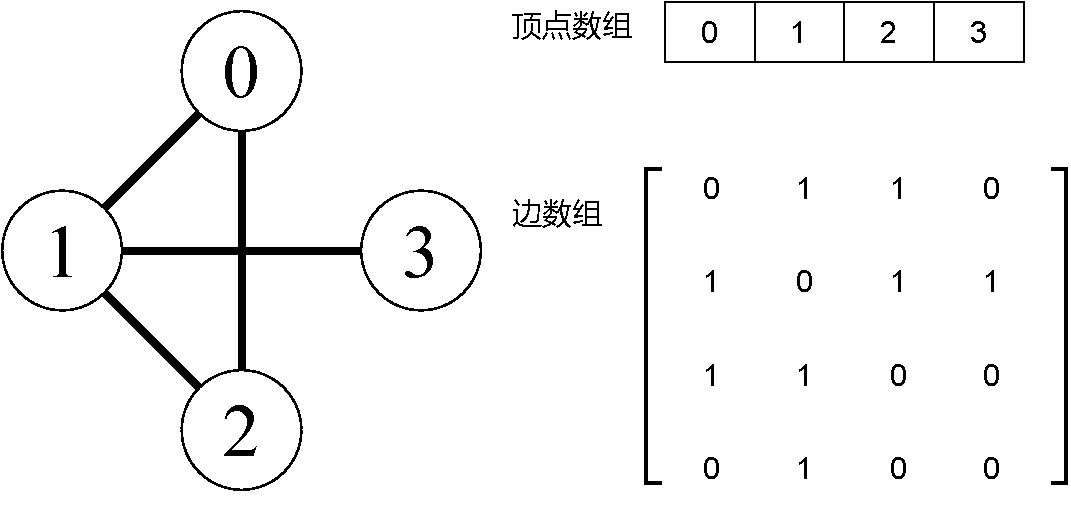
\includegraphics[width=7.3cm]{undirected_adj_mart.pdf}
        }
        \subfloat[有向图]{
            \label{pic:dir_adj_mart}
            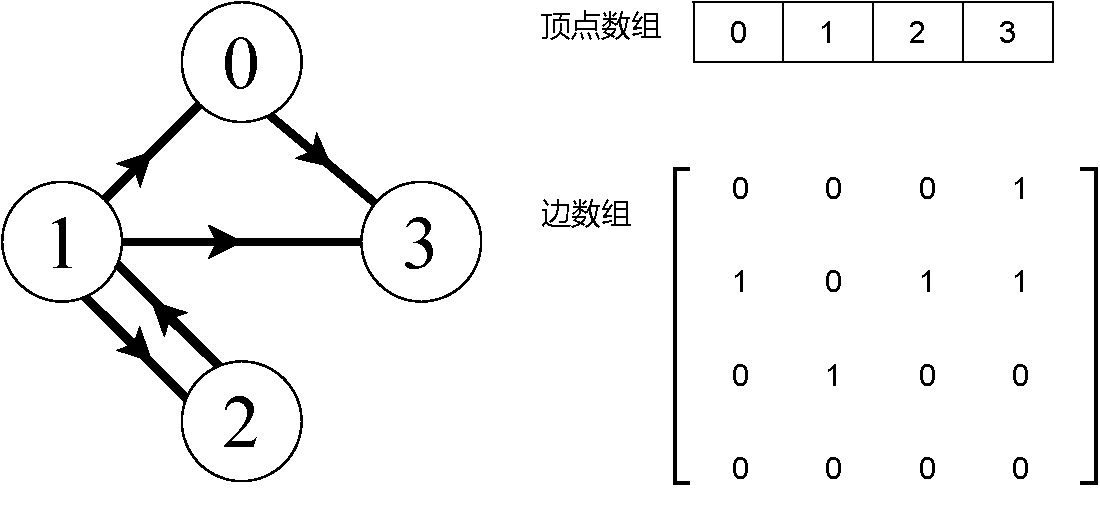
\includegraphics[width=6.41cm]{directed_adj_mart.pdf}
        }
        \caption{邻接矩阵}
        \label{fig:adj_mart}
    \end{figure}
    \item[(2)] 邻接表
    
        领接矩阵中即使两个顶点之间没有边,也会在矩阵中占据空间,对于边相对较少的稀疏图,使用邻接矩阵浪费很多存储空间。因此考虑对
    边使用链式存储的方式来避免空间浪费。领接表是由两部分组成。与邻接矩阵相同的是顶点也使用一维数组存储。而边信息不在使用二维数组,
    每个顶点的所有连接边存储为线性表,由于领接点的个数不定,采用单链表存储,无向图称为顶点的边表,有向图则称为顶点的出边表。

    \begin{figure}[h]
        \subfloat[无向图]{
            \label{pic:undir_adj_list}
            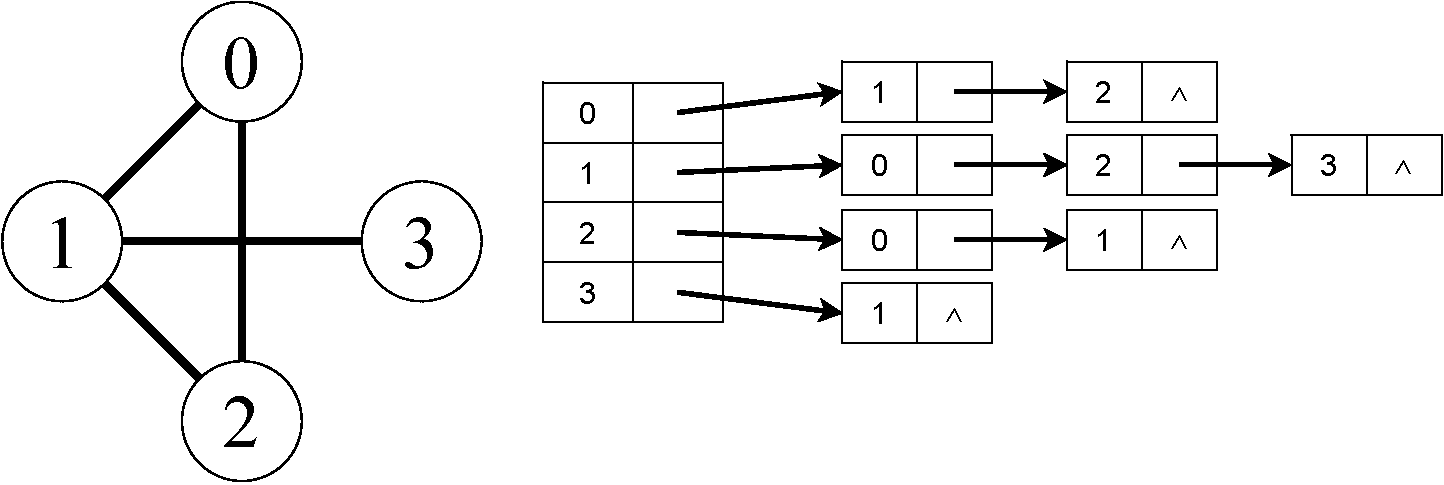
\includegraphics[width=7.3cm]{undirected_adj_list.pdf}
        }
        \subfloat[有向图]{
            \label{pic:dir_adj_list}
            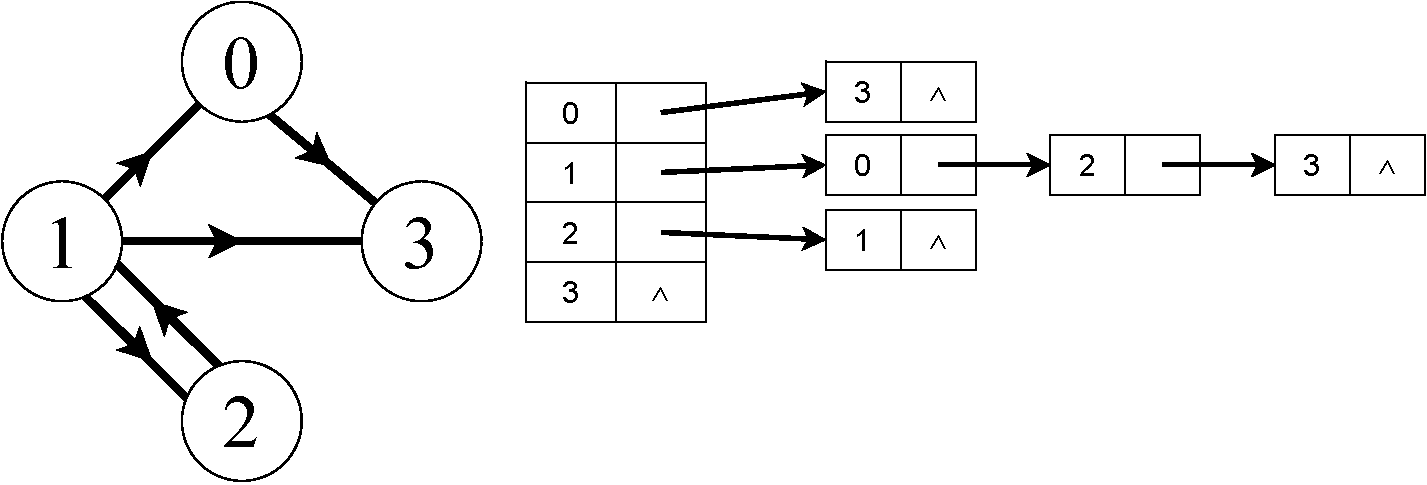
\includegraphics[width=6.41cm]{directed_adj_list.pdf}
        }
        \caption{邻接表}
        \label{fig:adj_list}
    \end{figure}
        
        在有向图中,每个顶点的出边表结点个数为该顶点的出度,若要求顶点的入度,则需遍历整个邻接表。有时为了便于求有向图中顶点的入度,
    会建立一个有向图的逆邻接表。逆邻接表与邻接表相反,每个顶点建立一个入边表。
    
    \item[(3)] 十字链表
    
        邻接表的缺陷是想要获取某个顶点入度需要遍历整个图,虽然可以通过再建立一个逆邻接表来弥补,但这样会带来更多的冗余存储消耗。十字链表
    将二者整合在一起解决这个问题。十字链表能够方便地求得顶点的出度和入度。而且创建十字链表的时间复杂度和邻接表相同。因此有向图使用十字链
    表存储是常见方法。

    \begin{figure}[h]
        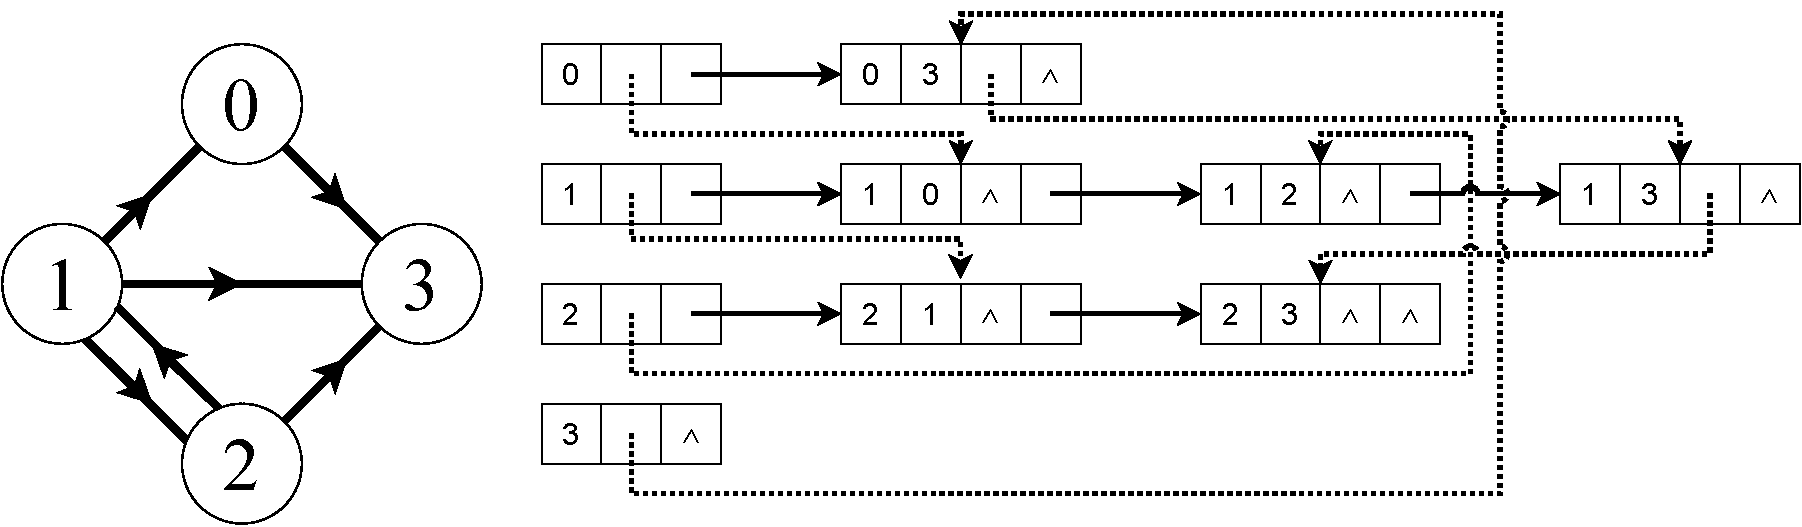
\includegraphics{directed_orthogonal_list.pdf}
        \caption{十字链表}
        \label{fig:orthogonal_list}
    \end{figure}

    \item[(4)] 边集数组
        边集数组将每个条边的起点下标、终点下标和属性存储为顺序数组,其中属性可以为空。边集数组是以边为核心的存储结构,在边集数组中要查找一个顶点的度需要
    扫描整个边数组。它更适合对边依次进行处理的操作,而不适合针对顶点的操作。
    
    \begin{figure}[h]
        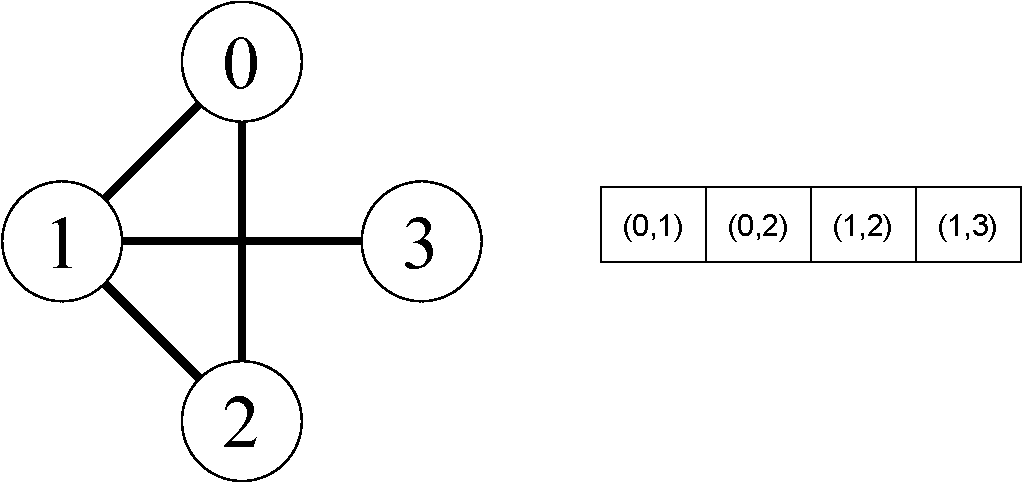
\includegraphics{edges_array.pdf}
        \caption{边集数组}
        \label{fig:edges_array}
    \end{figure}

\end{enumerate}

\subsection{图的常用算法}
    图的算法提供了最有效的分析图数据结构的方法,它们描述了如何处理图以发现一些定性或者定量的结论。
图算法基于图论,利用顶点之间的关系来推断复杂系统的结构和变化。
\begin{enumerate}
    \item[(1)] 图的遍历
    图的遍历是指从图中的某一个顶点出发,按照某种搜索方法沿着图中的边对图中的所有顶点访问一次且仅访问一次。
按照访问顶点的顺序主要分为两类:广度优先搜索和深度优先搜索。广度优先搜索是一种分层的访问过程,从起始顶点出发
优先访问起始顶点的所有邻域,再访问邻域顶点的邻域,以此类推直到访问所有顶点。深度优先搜索选择访问过的顶点的任
意邻域顶点,尽可能的沿着边进行访问,直到不能继续前进则回溯。
    
    \item[(2)] 最短路径
    最短路径是在两个顶点之间寻找最短的路径,主要算法有Dijkstra算法、Floyd-Warshall算法。Dijkstra算法解决
单源最短路径,求解给定顶点到任意其他顶点间的最短路径。该算法根据最短路径的最优子结构性质,从起点开始不断更新
每个顶点到起点的最短路径,遍历完毕后可得起点到每个顶点得最短路径。Floyd-Warshall算法解决任意两点间的最短路
径,如果从一个点到另一个点的直接路径不是最短的,那最短路肯定要经过第三个点。所以就用所有的点都当一次中间点
插入到当前两点间最短路径中,来判断是不是任意两点之间经过中间点路程会减小。

    \item[(3)] 最小生成树
    最小生成树是在加权连通图里搜索边子集所构成的树,该树包括了图里的所有顶点,且其所有边的权值之和为最小。
主要有Prim算法、Kruskal算法。Prim算法维护一个顶点集和一个边集,顶点集任意加入一个图中顶点作为初始值,边集初始
为空,然后不断选择图中权值最小且其中一端在顶点集中的边,将边加入边集,将另一端加入顶点集。直到顶点集包含图中所有
顶点。Kruskal算法把所有的边按照权值先从小到大排列,接着按照顺序选取每条边,如果这条边的两个端点不属于同一集合,
那么就将它们合并,直到所有的点都属于同一个集合为止。

\end{enumerate}

\subsection{图数据的应用领域}
\label{subsec:graph-app}


    图数据能够建模多种领域的数据。很多问题能在图论支撑下借助图相关的算法得到高效解决,例如图形着色,网络路由,网络流等
。研究图计算高效处理大规模图数据,能推动社交网络分析、语义web分析、生物信息网络分析、自然语言处理和MLDM等新兴应用领域
的发展。此外图计算的应用领域还包括:流量图,用来监控和应对道路事故,分析网络安全,网页搜索[3];生物图,进行研究药物模
型(例如蛋白质相互作用),预测疾病爆发;社交图,对舆情分析,推荐人或产品和信息流跟踪等。
\begin{table}
    \label{tab:graph-app}
   \caption{图数据的典型应用}
   \begin{tabular}{|c|c|c|c|}
    \hline
    数据 & 顶点 & 边 & 典型问题\\
    \hline
    蛋白质结构网络 & 氨基酸 & 接触残基 & 氨基酸模块化结构发现、蛋白质互相作用~\cite{Spontaneous}\\
    \hline
    社交网络 &用户个体 & 关注关系 & 社会角色划分、好友推荐、圈子探测~\cite{Role} \\
    \hline
    Web连接结构 &Web页面&页面之间的超链接 & PageRank页面排名~\cite{PageRank}\\
    \hline
    软件网络& 计算节点& 计算节点之间的互联 & 软件调用规划~\cite{SoftwareHomology}\\
    \hline
   \end{tabular} 
\end{table}

    从表中可以看出图数据的运用领域广泛。在这些领域中,有很多值得探究的具体问题:如在生物信息学中,将氨基酸建模为顶点
将接触残基建模为边,形成蛋白质结构网络,使用频繁子图挖掘可以从中发现大量出现的氨基酸模块化结构。又如在社交网络中,
用户看作顶点用户之间建立的关系看作边,可以通过大度数顶点寻找权威,通过最短路径长度可以获知两个用户之间人脉距离。
上述问题中除了需要处理实体携带的信息,更多地需要从图的拓扑结构进行分析。这反映了图数据不同于其他数据的一个
特点:在图数据中的“关系”至关重要,不仅仅是顶点或者边的属性能够表达信息,图的拓扑结构本身也蕴含着知识。图挖掘的目的正是
为了从图数据结构中发现知识。

\section{图挖掘技术}
\label{sec:graph-mining}

    图挖掘是从海量的图模型数据中发现和提起有用知识和信息的过程。图数据注重事物之间的联系,图的结构体现了这种联系的总体
特征。研究者常用集聚系数、三角数量、闭合三角比值等等指标来衡量一个图数据集。这些指标的获得需要在图数据集中寻找一些特定
的子结构,如三角形、团、路径等等。发现这些子结构的过程称为模式挖掘,这些子结构被称为模式。

\begin{table}
    \label{tab:graph-parameter}
   \caption{图数据集的典型指标}
   \begin{tabular}{|c|c|}
    \hline
    指标 & 含义\\
    \hline
    集聚系数 &  每个顶点连接的邻域顶点之间边的数量,除以这些顶点之间可以连出的最大边数(即团)\\
    \hline
    社交网络 & 三角形数量 \\
    \hline
    闭合三角比值 & 三角形的数量与所有连通三点组(即三角形和三顶点路径)的总量之比\\
    \hline
   \end{tabular} 
\end{table}

    模式挖掘是一个经典的图挖掘问题,被认为是研究最多的问题之一。图模式挖掘问题针对的是标记了顶点和边的输入图。模式是一
个任意的图结构,模式挖掘算法旨在发现输入他中所有模式与匹配的子图。如下:

    \textbf{图同构}:如果两个图$G$和$H$的顶点和边之间存在一对一映射,则称$G$和$H$同构,在有向图中边还需要保持方向的一致。
更非正式地说,如果我们忽略单个顶点之间的区别,同构指的是两个图具有相同边结构和相同拓扑。
    
    \textbf{子图}:$G$的子图$G'$有$V(G') \subseteq V(G), E(G') \subseteq E(G)$。子图中的每个节点也是父图中的一个节点,
子图中的每条边都是父图中的一条边。另外,当$G'$满足$\forall (u,v) \in E(G') \leftrightarrow (u,v) \in E(G)$时,称$G'$为
诱导子图。即$E(G')$包含了$E(G)$中所有两端连接在$V(G')$的边。

    \textbf{匹配和频率}:匹配指的是给定一个模式$P$,图$G$中能够找出子图$G'$与$P$同构。$P$在$G$中的频率是不同的$G'$的数量,
如果两个匹配不共享所有节点和边,则认为它们是不同的。
    
    模式挖掘集中在枚举满足用户指定特征的所有模式$P$的上。在输入数据集$G$上列出给定的模式$P$的子图,这些子图也称为$P$在$G$中
的嵌入。然后通过评估筛选出满足条件的模式,比如出现次数大于给定阈值。

    典型的模式挖掘应用包括以下几类:
\begin{enumerate}
    \item[(1)] 子图查询
    
    给定两个图$G$和$P$,确定$G$中是否包含与$P$同构的子图,也可以更简单地看作计算$H$出现次数是否大于零。
对于一般图,这是一个已知的NP完全问题。这项任务与图同构问题密切相关~\cite{Isomorphism},许多子图查询方法依赖于找到$G$中所有包含的子图,
然后检查找到的子图是否与$H$同构。一些子图查询算法使用了著名的nauty工具~\cite{Nauty}来辨别子图的类型~\cite{Towards,GTries,FANMOD}。

    \item[(2] 网络主题挖掘
        
    如果有某种子图,在图$G$中在出现次数高于其在随机图$R$中出现次数,则称为主题~\cite{Motifs},网络主题用于发现图数据中的局部规律。
常用的随机图$R$与图$G$保持相同度序列,通过多次随机交换$R$中的任意两条边其中一个顶点来实现,这样保持了度数不变。重要度来表现一个主题是否
经常出现的指标,对于每一个主题计算图$G$中主题个数$N_i^{real}$和随机图中主题个数$N_i^{rand}$,可得Z=score统计量
$Z_i\frac{N_i^{real}-N_i^{rand}}{N_i^{real}}$,标准化后得到重要度指标(significance profile)$SP_i=\frac{Z_i}{\sum_{k=1}^{n}Z_j}$
可以用来比较不同的主题相对重要程度。

    \item[(3)] 频繁子图挖掘

    找到在图$G$出现频率高于给定阈值的所有子图结构,最终根据频率对子图结构进行排序。与主题不同,频繁子图挖掘
不需要比较随机图,直接在图$G$中搜索。通常频繁子图挖掘问题有两种分支:输入一组图数据集在其中寻找其中大量共同出现的子图;
输入单个大的图数据搜索其中频率较高的子图~\cite{SurveyFSM}。主要方法是从最简单的模式(例如,一个顶点或一条边)开始在$G$中统计出现个数,
筛选掉频率小于$K$的模式。然后,通过再添加一个顶点或边来扩展模式,并重复统计个数然后筛选的步骤,候选集为空。这里运用了向下封闭属性进行剪枝,
即一个模式出现频率如果大于$K$,该模式的子图频率也一定大于$K$。

\end{enumerate}

    在模式挖掘中,子图同构是基础,网络主题挖掘、频繁子图挖掘更进一步要求统计同构发生的次数,模式计数算法正是其中的重点。子图同构本身就是
一项NP完全任务,想要再此基础上对寻找到的模式进行计数则更加困难。随着图数据集规模日趋庞大,顶点和边数量大于$10^9$的图数据愈来愈普遍,精确
计算模式出现次数的开销越来越难以接受,因此很多研究寻求使用近似计算理论来进行模式挖掘。下一章将介绍近似计算相关理论。

\section{近似计算技术}
\label{sec:approximate}
    
    目前广泛应用大数据处理框架主要作用是大规模数据分析,以批处理计算为主,其实时性需求得不到满足。在大数据应用场景下,数据价值会随着
时间的流逝而衰减,因此期望能够尽快对最新的数据做出分析并给出结果,并实时展示,以达到实时计算。但随着数据规模的日益庞大,计算数据的时
间却变得越来越长。为了缓解这个矛盾,提出了近似计算技术,它基于直观的考虑:在执行精确计算需要大量的计算资源,允许选择性的近似处理,达成
可以接受的精度损失和大规模的计算时间节约。有效的近似技术需要明智的选择近似策略,否则可能导致难以接受的质量损失。

\subsection{数据采样}
\label{subsec:sample}
    近似计算最常用的手段是是对查询或算法处理的输入进行采样。给定一个数据集(有时我们称之为“总体”),首先从数据集中随机选择少量元素。
然后对样本计算一些统计数据,例如样本、均值和方差。最后,这些统计信息用于估计查询结果的值,并提供估计精度的界限。
数据采样通过缩减数据集规模达到减少执行时间的效果,并且采样方法可以指定执行时间限制,通过预测在限制时间内处理能力来决定
样本的大小。
    
\subsubsection{数学模型}
\label{subsubsec:math-model}
    样本是通过某种随机过程从原始数据集中选择的一组元素,采样过程可按以下方式进行建模。用$t_j$表示数据集中的第$j$个元素
,用$X_j$表示样本中第$j$个元素出现次数的随机变量。$X_j$的样本空间是非负整数,即$X_j = \{x_j \ge 0\}$。不同的$X_j$取值
表示了不同的采样行为,比如$x_j = 0$表示$t_j$没有被采样到,否则$t_j$被采样到$x_j$次。通过改变采样过程(有替换、无替换、有偏差、
无偏差等),可以改变了各种$X_j$的统计特性,也改变了采样过程的统计特性。例如,在伯努利采样中,$t_j$采样概率为$p$,
样本空间为$X_j = \{0, 1\}$,即$P(X_j = 1) = p, P(X_j = 0) = 1-p$。
    将$X_j$和$t_j$应用于近似问题,需要构造可以用来估计近似结果的估计量。估计量$Y$可以看作一个函数$F$,将所有控制采样过程的随机
变量和所有数据元素参数化:
\begin{equation*}
    Y=F((t_1,X_1), (t_2,X_2),\ldots,(t_n,X_n))
\end{equation*}
通常$X_j = 0$的项表示没有被采样可以忽略:
\begin{equation*}
    Y=F(\ldots,(t_{i-1},X_{i-1}), (t_i,0),(t_{i+1},X_{i+1}),\ldots)=F(\ldots,(t_{i-1},X_{i-1}),(t_{i+1},X_{i+1}),\ldots)
\end{equation*}
    $Y$是一个由函数$F$生成的新随机变量。通过对这个随机变量进行试验(即,执行采样过程以获得每个$x_j$,然后对结果应用$F$),我们可以
得到近似计算的估计值。

\subsubsection{估计质量}
\label{subsubsec:quality}
    通常采样方法用$Y$的偏差$bias(Y)$和方差$\sigma^2(Y)$来量化效用和准确性。
\begin{equation*}
    bias(Y)= E[Y]-Q
\end{equation*}
其中$E[Y]$是$Y$的预期值,$Q$是精确计算结果。偏差表示了$Y$平均值与$Q$的距离。当$bias(Y)=0$,称$Y$是$Q$的无偏估计。
\begin{equation*}
    \sigma^2(Y)= E[(Y - E[Y])^2]= E[Y^2] - E^2[Y]
\end{equation*}
方差表示Y围绕其平均值的差距,意味着估计量的可变程度。如果$Y$拥有较低的偏差和方差,则认为$Y$由较高的估计质量。

    所以很多用户还要求在给出估计结果的同时提供置信区间,通常表述为:“精确计算结果在$[l,h]$区间范围内的概率为$p$”。

    \textbf{中心极限定理}。中心极限定理表明对于独立的随机变量,即使变量本身不是正态分布,其归一化和的极限趋向于
正态分布。在数据采样中随着从分布中提取的独立样本数量接近无穷大,观察到的分布均值和样本均值之间的差异越来越接近正态分布。
对于$Y$有:
\begin{equation*}
    \lim_{n\rightarrow\infty}Y= N(E[Y], \sigma^2(Y))
\end{equation*}
当$Y$是$Q$的无偏估计时,可以假设估计误差也是正态分布:
\begin{equation*}
    Q-Y \approx N(0, \sigma^2(Y))
\end{equation*}
选择不同的置信度,可以确定置信区间的两个端点$lo$和$hi$:
\begin{equation*}
    p=\int_{lo}^{hi}f_N(x)dx
\end{equation*}
其中$f_N$是$N(0, \sigma^2(Y))$的概率密度函数,这个式子表示$lo \le Q-Y \le hi$的概率为$p$。令$l=lo+Y$、$h=hi+Y$,
则$Q$在$[l,h]$区间范围内的概率为$p$。

    以置信度0.95为例,有:
\begin{equation*}
    \int_{-1.96\sigma(Y)}^{1.96\sigma(Y)}f_N(x)dx=0.95
\end{equation*}
则可以称$Q$在$[Y-1.96\sigma(Y), Y+1.96\sigma(Y)]$范围内的概率为95\%。

    根据统计理论,中心极限定理具有很大的普遍性,即便在样本数量不是非常庞大,假设$Y$误差服从正态分布依然是安全的。

    \textbf{切比雪夫界}。在数据采样的运用中,如果回避对于数据分布的假设,可以采用切比雪夫不等式,它相比中心极
限定理更宽松。对于无偏估计$Y$有:
\begin{equation*}
    Pr\left[\vert Q-Y \vert \ge p^{-\frac{1}{2}}\sigma(Y) \right] \le p
\end{equation*}
可以称Q在$\left[ Y-p^{-\frac{1}{2}}\sigma(Y), Y+p^{-\frac{1}{2}}\sigma(Y) \right]$区间内的概率为$p$。

    \textbf{霍夫丁界}。当$Y$的方差难以计算时,可以采用霍夫丁不等式来估计置信区间,它适用于$Y=\frac{1}{n}\sum_iX_i$
且$X_i$值有界的情况:
\begin{equation*}
    Pr\left[\vert Y-E[Y] \vert \ge d \right] \le 2exp\left(-\frac{2d^2n^2}{\sum_i(lo_i-hi_i)^2}\right)
\end{equation*}
其中$lo_i$和$hi_i$是每个$X_i$值域的上下界,实际运用中,常用所有$X_i$中的最大值$MAX(X_i)$最小值$MIN(X_i)$来近似
处理$\sum_i(lo_i-hi_i)^2 \approx n(MAX(X_i) - MIN(X_i))^2$。霍夫丁界通常更为宽松。

    \textbf{切尔诺夫界}。切尔诺夫界与霍夫丁界密切相关,适用于$Y=\frac{1}{n}\sum_iX_i$但$X_i$取值只为0或1的情况。
切尔诺夫界不直接构造基于采样的置信区间,但它们为各种采样方法构造了精度证明的重要工具。

\subsubsection{数据采样的优点和缺陷}
\label{subsubsec:advantages-drawbacks}
    数据采样是一种简洁的近似计算的手段,从概念上很容易理解从数据集中随机选择元素的思路,然后在样本上放大计算结果以猜测
整个数据集的结果。数据采样允许在计算开始后构造样本而不需要提前生成,因此具有灵活性,可以实时地根据选取样本的多寡来权衡
精度和执行时间。但数据采样往往对有歪斜的数据集比较敏感,数量稀少而又包含异常值的数据元素可能会导致估计结果质量较差。

% 本文也利用这种思想,预先对图数据集的幂律分布进行分析,建立度数序列等等概要信息,优化邻域采样过程。

\section{图近似模式挖掘技术}
\label{sec:graph-approximate}
    近似计算技术是大数据分析中取得很多成功的方法,因此很多研究探索在图模式挖掘中运用类似的技术。与其他领域中近似
计算相同,近似模式挖掘也主要使用数据采样策略,其主要思想是将图中的边建模为流并从中采样模式的实例,然后使用采样
概率来估计模式出现次数。研究者提出了多种基于不同的采样方法的模式挖掘技术。

\subsection{基于均匀采样的模式挖掘}
\label{subsec:uniform}
    均匀采样是对图数据边流$S$中的每一条边进行固定概率$p$的采样,本质是概率为$p$的$n$重伯努利实验,其中$n=|S|$。
当一条边$e(u, v) \in S$被采样到后,将$e$存储到$E_{samp}$。然后在$E_{samp}$执行精确模式挖掘算法,以三角形计数
为例。在$E_{samp}$中查找$N_{uv}=N_u \cap N_v$,$N_u$和$N_v$分别是顶点$u$和顶点$v$的邻接顶点集,$N_{uv}$
是$N_u$和$N_v$的交集,$N_{uv}$中每一个顶点都能够和边$e(u, v)$组成新的三角形。因此$e$加入到$E_{samp}$后,新
增三角形个数为$|N_{uv}|$。因为三角形中每一条边被采样到的概率为$p$,所以直观的认为三角形被采样到的概率应
为$p^3$,新增的估计三角形数量应为$|N_{uv}|*\frac{1}{p^3}$。当边流$S$中所有边遍历完毕后,可得出最终的估算结果。

\begin{figure}
	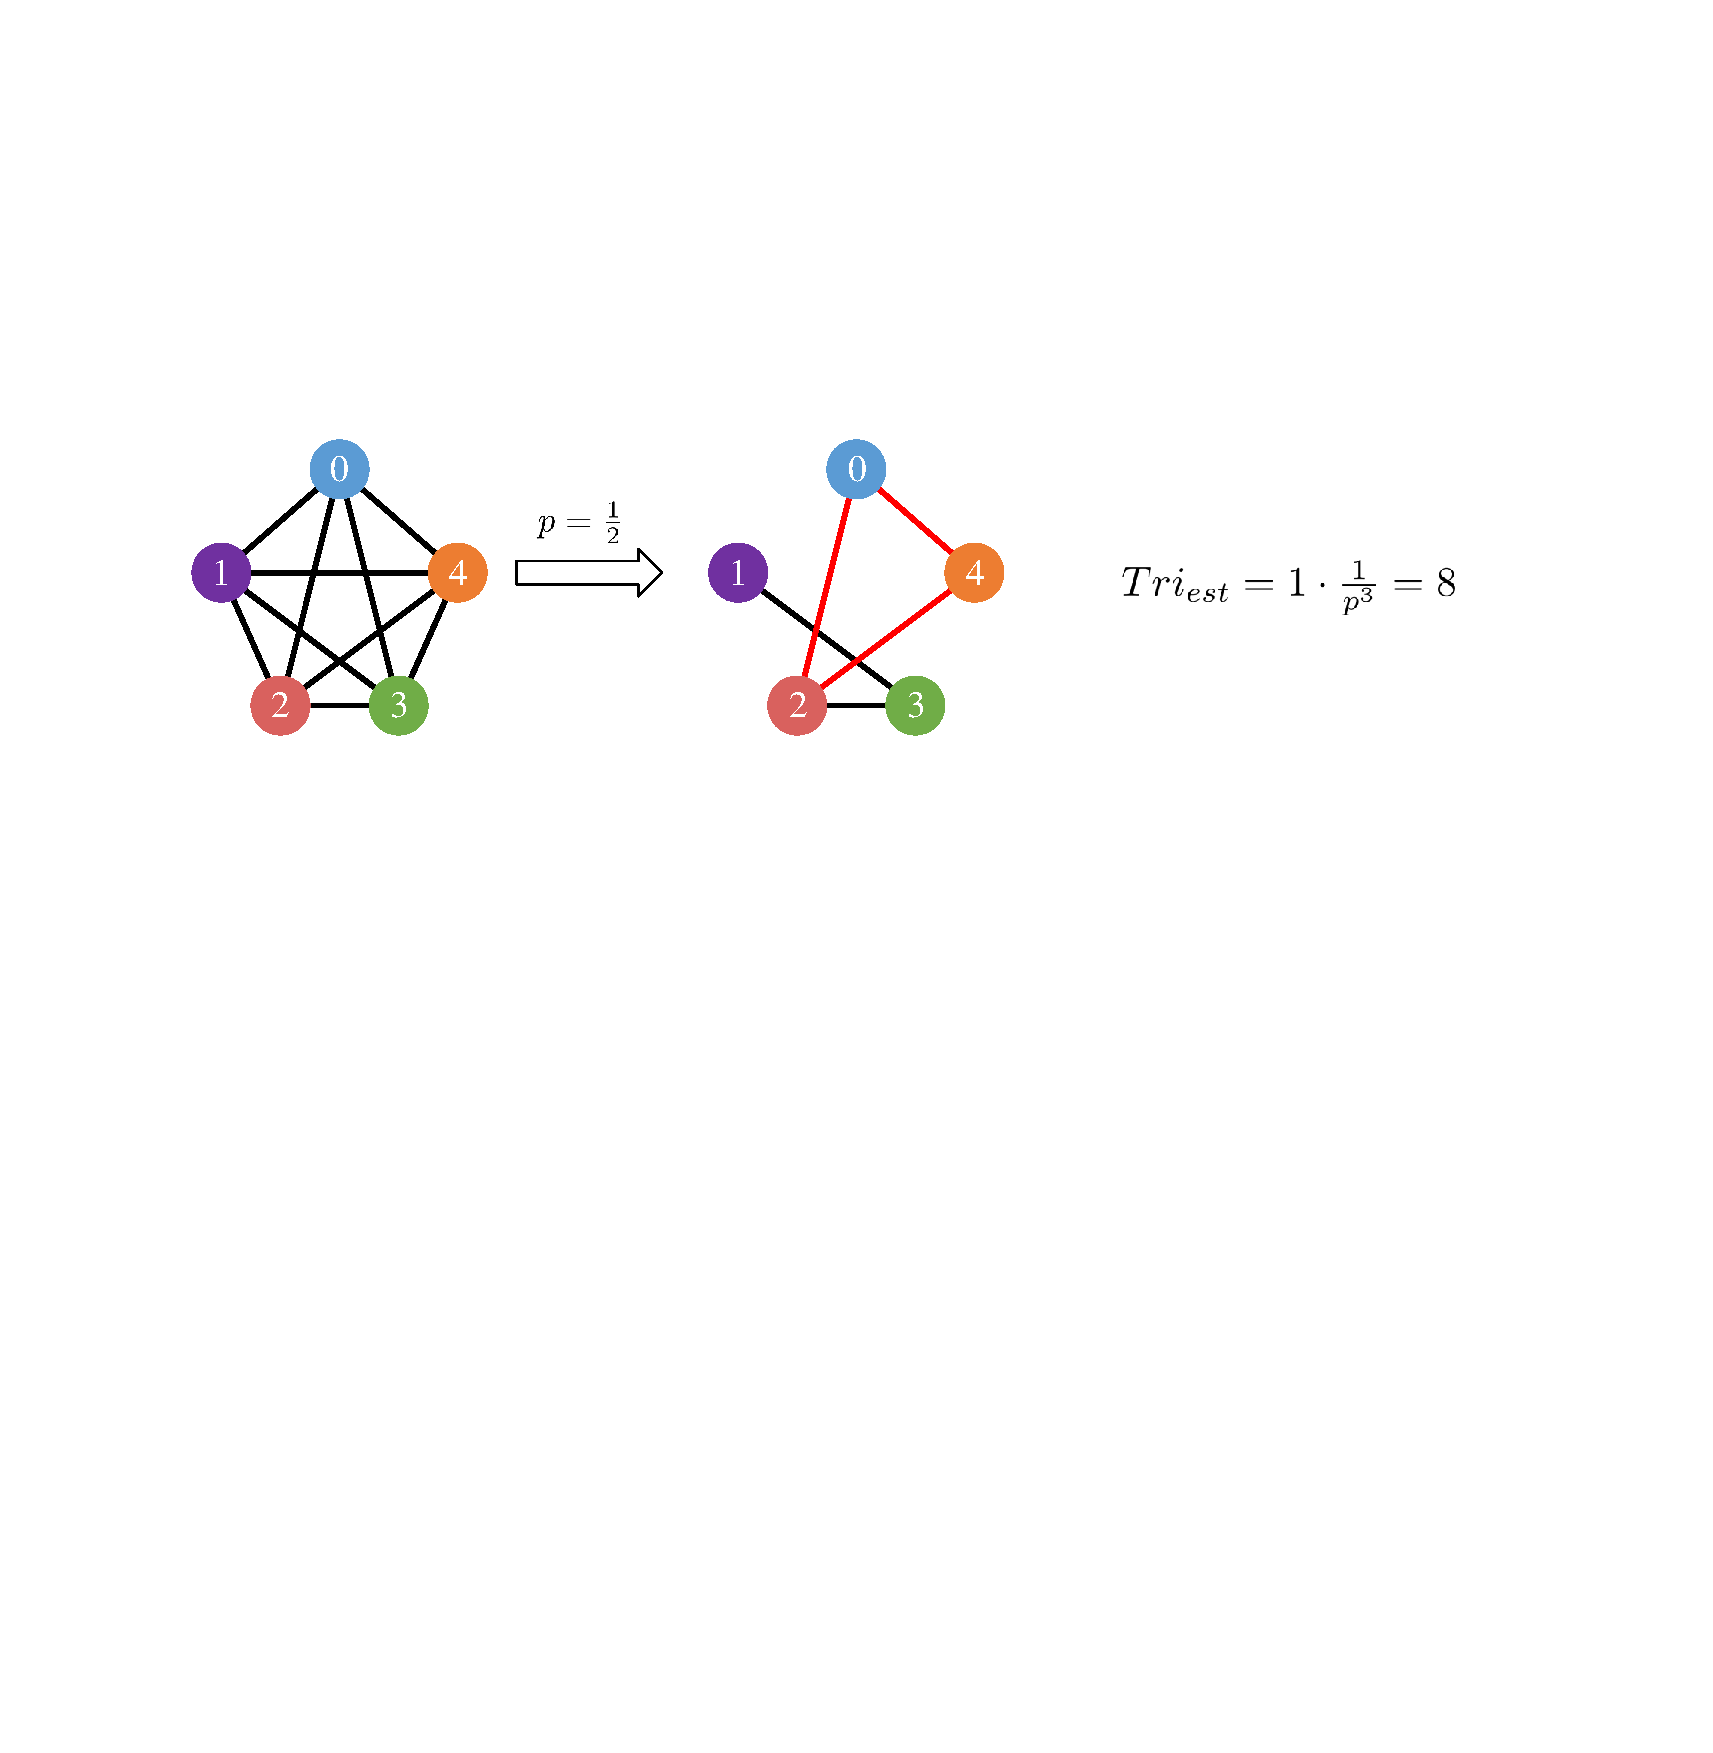
\includegraphics{uniform.pdf}
	\caption{均匀采样示例}
	\label{fig:uniform}
\end{figure}
     如图~\ref{fig:uniform}所示,在图$G$中以$\frac{1}{2}$概率均匀采样,在采样边$E_{samp}$中发现一个三角形,根据采样
概率估算形三角数量为8个。

\subsection{基于库采样的模式挖掘}
\label{subsec:reservoir}
    上一节\ref{subsec:uniform}中描述的均匀采样完整地存储所有被采样的边,当边的数量很大时,采样边的存储开销也会变得很大
,因此提出了库采样。库采样技术是通过限制样本规模来控制采样过程中的存储开销。下面给出一种基础方法的描述。

    在扫描图边流$S$中维护一个固定容量为$M$的库$E_{samp}$,访问在边流中第$i$条边$e_i$时,如果$i<=M$无条件地将边存储到库中,
而当$i>M$后以概率$\frac{M}{i}$进行采样如果$e_i$被采样到则随机替换掉库中一条边。这种采样方法可以看作在$i$条边中均匀地选
择$M$条边。每条边加入库中执行模式挖掘得出更新模式计数$\tau$,具体方法与\ref{subsec:uniform}中描述的过程类似,不同之处在于需要
挖掘出被替换掉关联的模式并从计数中减去对应数量。接着根据$\tau$估算原图中模式总数。

    挖掘的模式$p$的边数为$k$。当$i<M$,所有边都被存储到了$E_{samp}$中此时$\tau$为准确计数。当$k>MIN(i,M)$,$p$不可能被计数。
所以重点是当$k<M<i$时的$p$被计数的概率。设:
\begin{itemize}
    \item $I$是原图中任意一个与$p$同构的子图,$E_I$是$I$的边集且$E_I \subseteq S$。
    \item $\alpha$是边集的集合,$\alpha$中每个元素大小为$M$且包含$E_I$,$\alpha={A: |A| = M , E_I \subseteq A}$。
\end{itemize}
则有:
\begin{equation*}
    |\alpha|=\left(\begin{array}{c}
        i-k\\
        M-k
    \end{array}\right)
\end{equation*}
又对于任意一个大小为$M$的边集$A$,被采样到库中的概率为:
\begin{equation*}
    Pr(E_{samp}=A)=\left(\begin{array}{c}
        i\\
        M
    \end{array}\right)
\end{equation*}
$E_I$出现在$E_{samp}$中的概率:
\begin{equation*}
    \begin{aligned}
        Pr(E_I \subseteq E_{samp})&=Pr(E_{samp} \in \alpha)=\sum_{A\in\alpha}Pr(E_{samp}=A)\\
        &=\frac{\left(\begin{array}{c} i-k \\ M-k \end{array}\right)}{\left(\begin{array}{c} i \\ M \end{array}\right)}
    \end{aligned}
\end{equation*}
因此对原图中模式总数估计为$\frac{\tau}{Pr(E_I \subseteq E_{samp})}$。
 
\subsection{基于邻域采样的模式挖掘}
\label{subsec:neighbor}
    邻域采样是利用模式的连通性提出的一种采样方法,首先在边集中对一条边采样,然后后续从已采样边的邻域中添加更多边,
,直到边形成模式或者边流中不能再找出邻域。

    设图数据集的边流大小为$m$,模式$p$的边数为$k$。从图中以概率$Pr(l_1)=\frac{1}{m}$采样第一条边$l_1$。在出现于$l_1$之后的
边流中搜索$l_1$的邻域$N(l_1)$,从中以概率$Pr(l_2)=\frac{1}{|N(l1)|}$采样$l_2$。同样,在$l_2$后续边流中搜索$N(l_1) \cup N(l_2)$
并以概率$Pr(l_3)=\frac{1}{|N(l_1) \cup N(l_2)|}$采样$l_3$。以此类推,直到剩余最后一条边$l_k$,停止采样直接在剩余边流中检查是否存在
$l_k$能够与之前采样的边形成$p$的同构子图。如果是以$\frac{1}{Pr(l_1)*Pr(l_2)*\cdots*Pr(l_{k-1})}$估计原图中模式数量,否则估计为0。
邻域采样方法对边流执行一次上述过程称为运行了一个估计器,最终结果是多个估计器结果的均值。

\begin{figure}
    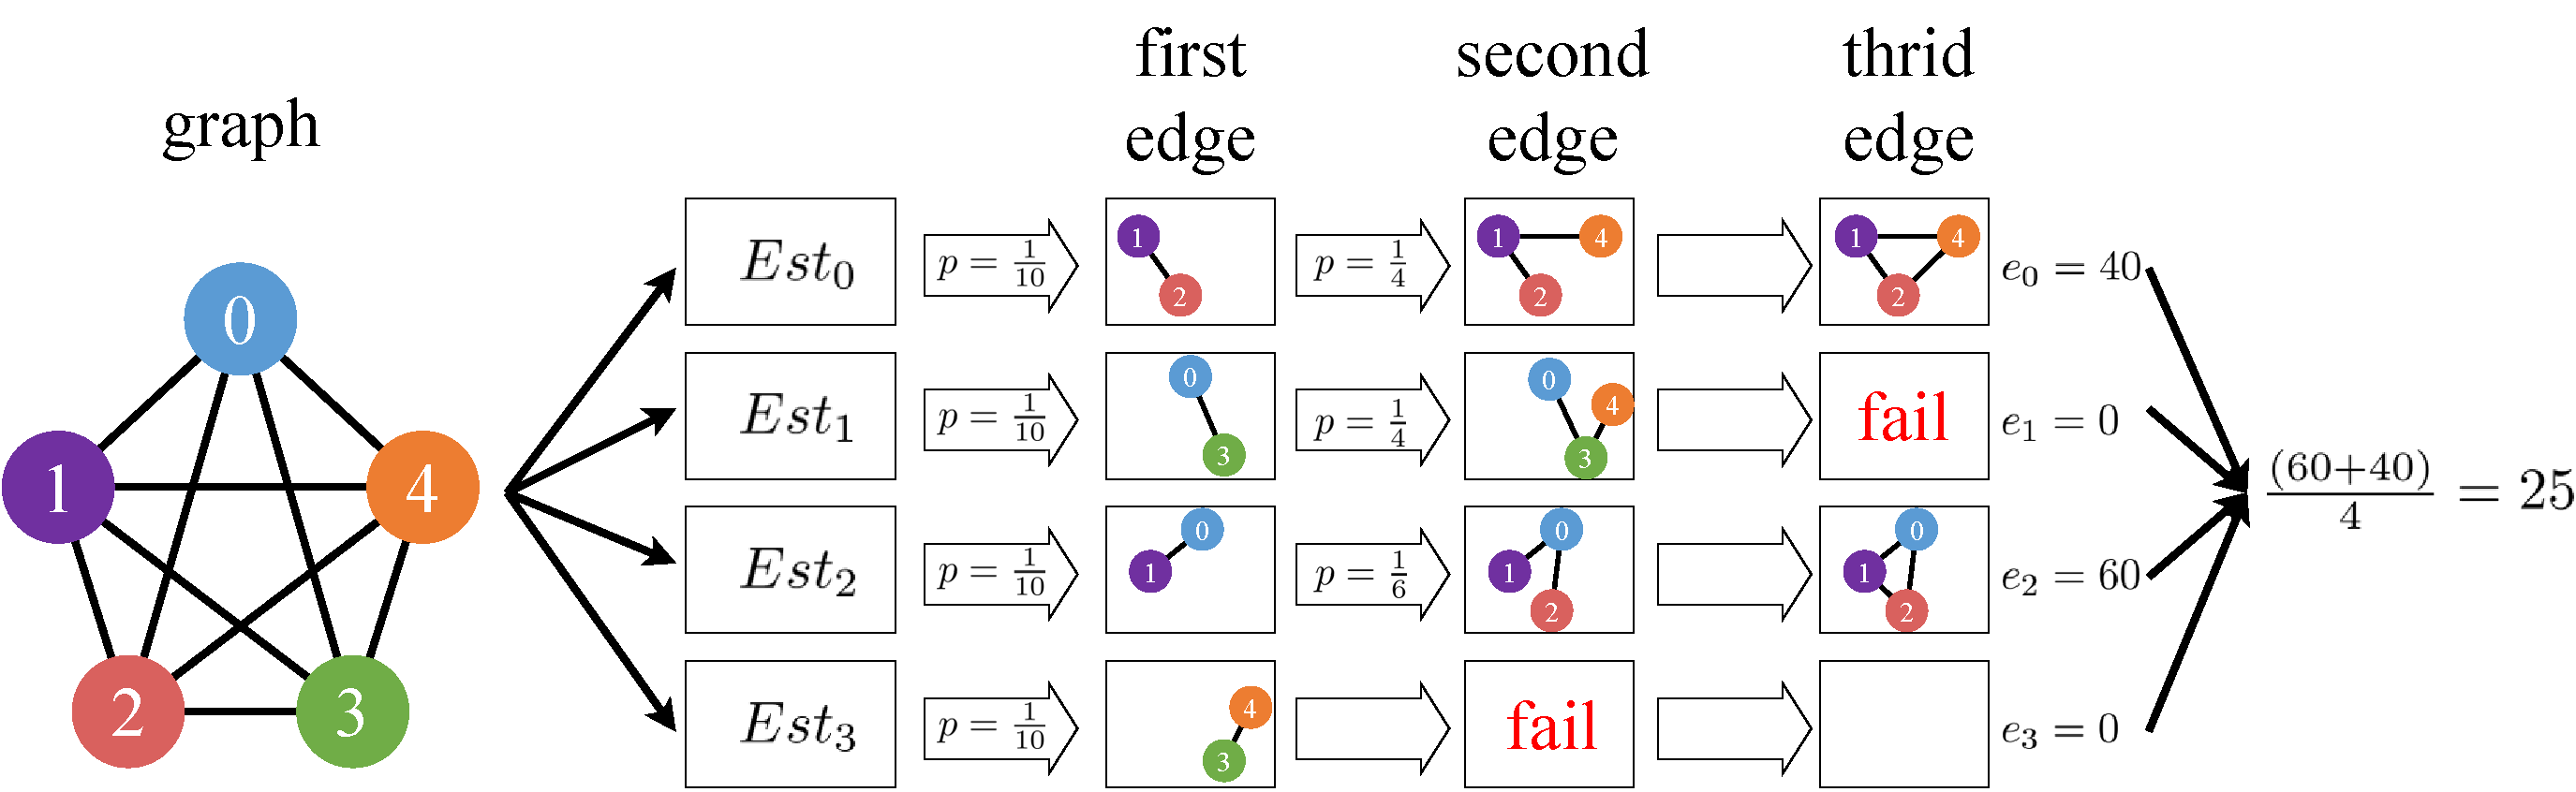
\includegraphics{tri_nei_samp.pdf}
	\caption{基于邻域采样的三角形计数示例}
	\label{fig:tri_nei}
\end{figure}
    在图\ref{fig:tri_nei}中展示了如何使用邻域采样方法进行三角形计数,这里使用了四个估计器。以第一个估计器为例,首先以$\frac{1}{10}$的概率
采样了边$(1,2)$作为$l_1$,在后续边流中邻域$N(l_1)={(1,3),(1,4),(2,3),(2,4)}$,值得注意的是$(0,1),(0,2)$也是$l_1$的邻边,但由于在边流中
出现早于$l_1$并未被计入$l_1$的后续邻域。接着以$\frac{1}{4}$的概率采样$(1,4)$作为$l_2$,最后在$N(l_1) \cup N(l_2) = {(2,3),(2,4)}$中检
测到$(2,4)$可以形成三角形,因此输出估计值40。而在第二个估计器中,$l_2$采样到(3,4)后续已经没有邻域,因此输出估计值0。最后使用四个估计器的均
值作为最终结果。
    
    邻域采样相较于均匀采样和库采样,考虑模式的连通性,从已有边的邻域中继续采样边要比从所有边中采样概率大很多,因此提高了估计精度、加快了采
样速度。并且多个估计器相互独立,可以得益于并行化执行。但是邻域采样方法单一的估计器计算结果方差很大,对运行需要大量的估计器来保证估计精度。
本文的模式近似挖掘方法基于邻域采样方法,目的是根据图的幂律特征对邻域采样方法进行优化。

\section{图的幂律性质}
\label{sec:pow-law-graph}
    近年来随着Web2.0、大数据、社交网络、机器学习和数据挖掘
(MLDM - MachineLearningand Data Mining)等技术的高速发展,很多领域抽象出来的图规模呈指数级增长。
图中边的数量可达到亿万级别,另外再加上自然图往往表现出非常倾斜的幂律分布power-law[2]特性,
对图计算带来了巨大挑战。
    \textbf{幂律分布}。幂律分布也常被称为重尾分布、帕累托分布、Zipfian分布等,是计算机科学应用中越来越常见的模型;例如,它们已被用于描述互联网图的文件大小分布
和出度入度分布。下面描述幂律分布的一些基础定义:

    如果:
\begin{equation*}
    Pr(X \ge x) \sim cx^{-k}, c > 0, k > 0
\end{equation*}
非负随机变量X被称为具有幂律分布,粗略来看,幂律分布描述了分布的尾部根据指数$-k$下降的情况。概率密度函数为:
\begin{equation*}
    f(x) = cx^{-k-1}, c > 0, k > 0
\end{equation*}
幂律分布在双对数坐标下为一条直线,这为辨别是否具有幂律提供了一个简单的经验测试方法:
\begin{equation*}
    lnf(x) = lnc-rlnx, c > 0, r > 0
\end{equation*}
幂律分布的重要特性是无标度性,使得幂律分布的数据能够在任何规模下都能保持整体特性。
\begin{equation*}
    f(ax) = (ca^{-k-1})x^{-k-1}=bf(x)
\end{equation*}

    \textbf{幂律图}。是指图的度数$d$和具有该度数的顶点$v_{\#}(d)$满足关系
\begin{equation*}
    v_{\#}(d)=c \cdot d^{-k}
\end{equation*}
该式表示了幂律图有大量具有极低度的顶点和少数具有相对高度的顶点。由于幂律图分体现了无标度性,可以使用小规模数据集得出整体数据的特性。
本文利用这一特性提出一种模式分布模型构建方法:根据少部分度数子图中模式分布,使用非线性回归拟合整体模式曲线。下面介绍非线性回归方法。

    \textbf{非线性回归}。非线性回归是回归分析的一种方式。寻找因变量和自变量之间的函数模型,该函数是自变量和一组参数的非线性
组合,非线性值指的是变量指数不全为1。非线性回归常使用高斯-牛顿迭代法,在每次迭代中不断修正参数值使残差平方和达到最小
输入一组观测数据${(x_0,y_0),(x_1,y_1),\ldots,(x_{n-1},y_{n-1})}$,设置函数基本模型$f(c;x)$,其中$\mathbf{c}=(c_0,c_1,c_{p-1})^T$表示需要回归的参数。
设$\mathbf{g}^{(0)}=\left(g_0^{(0)},g_1^{(0)},\ldots,g_{p-1}^{(0)}\right)$是参数的初始值。对于任意$x_i$,将$f(\mathbf{c};x_i)$在$\mathbf{g}^{(0)}$处作一阶
泰勒展开:

\begin{equation*}
    f(\mathbf{c};x_i)=f(\mathbf{g}^{(0)};x_i) + \sum_{k=0}^{p-1}\left[\frac{\partial f(\mathbf{c};x_i)}{\partial c_k}\right]_{\mathbf{c}=\mathbf{g}^{(0)}}\left(c_k-g_k^{(0)}\right)
\end{equation*}
则有:
\begin{equation*}
    y_i - f(\mathbf{g}^{(0)};x_i) \approx \sum_{k=0}^{p-1}\left[\frac{\partial f(\mathbf{c};x_i)}{\partial c_k}\right]_{\mathbf{c}=\mathbf{g}^{(0)}}\left(c_k-g_k^{(0)}\right)
\end{equation*}
令
\begin{equation*}
    y_i^{(0)}=y_i- f(\mathbf{g}^{(0)};x_i), D_{i k}^{(0)}=\left[\frac{\partial f(\mathbf{c};x_i)}{\partial c_k}\right]_{\mathbf{c}=\mathbf{g}^{(0)}}, b_k^{(0)}=c_k-g_k^{(0)}
\end{equation*}
有
\begin{equation*}
    y_i^{(0)} \approx \sum_{k=0}^{p-1} D_{i k}^{(0)} b_k^{(0)}, \quad(i=1,2, \ldots, n)
\end{equation*}
以矩阵形式表示:
\begin{equation*}
    \mathbf{Y}^{(0)} \approx \mathbf{D}^{(0)} \mathbf{b}^{(0)}
\end{equation*}
其中
\begin{equation*}
    \mathbf{Y}_{n \times p}^{(0)}=\left[\begin{array}{c}
        y_1-f\left(g^{(0)};x_0\right) \\
        \cdots \\
        y_n-f\left(g^{(0)};x_{n-1}\right)
        \end{array}\right], \mathbf{D}_{n \times p}^{(0)}=\left[\begin{array}{ccc}
        D_{00}^{(0)} & \cdots & D_{0 p-1}^{(0)} \\
        \vdots & & \vdots \\
        D_{n-1 0}^{(0)} & \cdots & D_{n-1 p-1}^{(0)}
        \end{array}\right], \mathbf{b}_{p \times 1}^0=\left[\begin{array}{c}
        b_0^{(0)} \\
        \vdots \\
        b_{p-1}^{(0)}
        \end{array}\right]
\end{equation*}
用最小平方法估计修正$\mathbf{b}^{(0)}$,并更新$\mathbf{g}^{(0)}$
\begin{equation*}
    \begin{aligned}
        &\mathbf{b}^{(0)}=\left(\mathbf{D}^{(0) T} \mathbf{D}^{(0)}\right)^{-1} \mathbf{D}^{(0) T} \mathbf{Y}^{(0)} \\
        &\mathbf{g}^{(1)} =\mathbf{g}^{(0)}+\mathbf{b}^{(0)}
    \end{aligned}
\end{equation*}
每轮迭代中检验残差平方和
\begin{equation*}
    SSR^{(s)}=\sum_{i=0}^n\left[y_i-f\left( \mathbf{g}^{(s)};x_i\right)\right]^2
\end{equation*}
当满足给定的允许误差率$K$,即满足
\begin{equation*}
    \left|\frac{S S R^{(s)}-S S R^{(s-1)}}{S S R^{(s)}}\right| \leq K
\end{equation*}
停止迭代,输出$\mathbf{g}^{(s)}$。

\section{本章小结}
\label{sec:theroy-summary}
    在本章中首先描述了图数据的基础理论以及实际运用。接着介绍了图挖掘的相关技术,图挖掘正是从图数据中挖掘知识。
然后分析了近似计算的相关技术以及近似技术在图模式挖掘中的运用。最后介绍了图的幂律性质和相关的数学分析方法。

\chapter{全文总结与展望}

\section{全文总结}

\section{后续工作展望}

\thesisacknowledgement
在攻读博士学位期间,首先衷心感谢我的导师XXX教授

\thesisappendix

\chapter{中心极限定理的证明}

\section{高斯分布和伯努利实验}


% Uncomment to list all the entries of the database.
% \nocite{*}

\thesisbibliography{reference}

%
% Uncomment following codes to load bibliography database with native
% \bibliography command.
%
% \nocite{*}
% \bibliographystyle{thesis-uestc}
% \bibliography{reference}
%

\thesisaccomplish{publications}

\thesistranslationoriginal
\section{The OFDM Model of Multiple Carrier Waves}

\thesistranslationchinese
\section{基于多载波索引键控的正交频分多路复用系统模型}

\end{document}
